\documentclass[english]{scrartcl}
\usepackage[T1]{fontenc}
\usepackage{listings}
\usepackage{hyperref}
\usepackage{graphicx}
\usepackage{color}
\usepackage{soul}
\usepackage{seqsplit}
\usepackage{multirow}
\usepackage{enumitem}
\usepackage{graphicx}
\usepackage{float}
\usepackage{amsmath}
\begin{document}
\section*{Assignment 7}
\subsection*{Task 7.1}
\begin{enumerate}
\item states:
\\$x_1$ - door1 is reward door, door2 is tiger door, 
\\$x_2$ - door1 is tiger door, door2 is reward door;
\item actions:
\\$u_1$ - open door1 and finish game, terminal action, 
\\$u_2$ - open door2 and finish game, terminal action, 
\\$u_3$ - listen, sensing action, gives measurement $\{z_1, z_2\}$ as result;
\item measurement space:
\\$z_1$ - noise behind the door1,
\\$z_2$ - noise behind the door2;
\item cost function (expected rewards):
\\$r(b,u_1)=p_1*r(x_1,u_1)+p_2*r(x_2,u_1)=p_1*(+200)+(1-p_1)*(-1000)$,
\\$r(b,u_2)=p_1*r(x_1,u_2)+p_2*r(x_2,u_2)=p_1*(-1000)+(1-p_1)*(+200)$,
\\$r(b,u_3)=-50$;
\item associated probabilities:
\\in state $x_1$ person gets $z_1$ with probability 0.2 and $z_2$ with probability 0.8, thus with probability 0.2 he thinks, that tiger is behind the door1 and changes state to $x_2$,
\\in state $x_2$ person gets $z_1$ with probability 0.8 and $z_2$ with probability 0.2, thus with probability 0.2 he thinks, that tiger is behind the door2 and changes state to $x_1$.
\end{enumerate}
Whole scheme is depicted in the Figure \ref{fig:7-1}.

\begin{figure}[h]
\centering
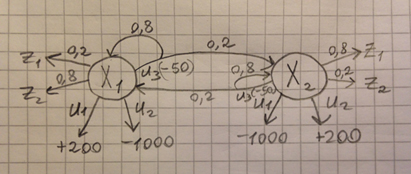
\includegraphics{./7-1}
\caption{POMDP scheme}
\label{fig:7-1}
\end{figure}

\subsection*{Task 7.2}
Cumulative reward (cost) of the sequence "Listen, listen, open door1" is: 
$$R=r(b,u_3)+r(b,u_3)+r(b,u_1)=$$
$$=-50-50+(+200)*p_{1}+(-1000)*(1-p_{1})=-1100-800p_1$$ where $p_1$ is probability of being in $x_1$
\\Person choose action $u_{1}$ anyway, independently of the measurement from $u_{3}$, thus we just sum up doubled cost of doing $u_{3}$ and expected reward after doing $u_{1}$.

\subsection*{Task 7.3}
Cumulative reward (cost) of the sequence "Listen, then open the door for which you did not hear a noise" is:
$$R=r(b,u_3)+p_1*(0.8*200+0.2*(-1000)) + (1-p_1)*(0.8*200+0.2*(-1000))=$$
$$=-50-40p_1-40+40p_1=-90$$
\\Person acts accordingly to the measurement after committing $u_{3}$, thus we sum up cost of $u_3$ and expected reward depending on measurement - it will be the same for $x_1$ and $x_2$, with probability 0.8 the person opens door with reward and with probability 0.2 - with tiger.

\subsection*{Task 7.4}
For time horizon 1
\[
    V_1(b)=max\left\{
                \begin{array}{ll}
                  -1000*p_1+200*(1-p_1)\\
                  200*p_1-1000*(1-p_1)\\
                  -50 \ // \ may \ discard
                \end{array}
              \right.
  \]
 depicted 
\\$p(z_1|x_1) = 0.2$ and $p(z_1|x_2)=0.8$. Getting measurement $z_1$ changes probabilities $p_1$ and $p_2=1-p_1$:
$$p_1^\prime=\frac{0.2p_1}{p(z_1)}$$
$$p_2^\prime = (1-p_1)^\prime = \frac{0.8(1-p_1)}{p(z_1)}$$
$p(z_2|x_1) = 0.8$ and $p(z_2|x_2)=0.2$. Getting measurement $z_2$ changes probabilities $p_1$ and $p_2=1-p_1$:
$$p_1^\prime=\frac{0.8p_1}{p(z_2)}$$
$$p_2^\prime = (1-p_1)^\prime = \frac{0.2(1-p_1)}{p(z_2)}$$
For expected belief after measurement:
\[
    V_1^\prime(b)=max\left\{
                \begin{array}{ll}
                  -1000*0.2*p_1+200*0.8*(1-p_1)\\
                  200*0.2*p_1-1000*0.8*(1-p_1)
                \end{array}
              \right. + 
  \]
  \[
              max\left\{
                \begin{array}{ll}
                  -1000*0.8*p_1+200*0.2*(1-p_1)\\
                  200*0.8*p_1-1000*0.2*(1-p_1)
                \end{array}
              \right. = 
  \]
  \[
     =max\left\{
                \begin{array}{ll}
                  -1000*p_1+200*(1-p_1)\\
                  -40*p_1-40*(1-p_1)\\
                  -760*p_1-760*(1-p_1) \ // \ may \ discard\\
                  200*p_1-1000*(1-p_1)
                \end{array}
              \right.
  \]
$u3$ potentially changes state, so, knowing that $p(x_1|x_1,u_3)=0.8$, $p(x_1|x_2,u_3)=0.2$, $p(x_2|x_1,u_3)=0.2$ and $p(x_2|x_2,u_3)=0.8$, we get:
$$p_1^\prime=0.8p_1+0.2(1-p_1)=0.6p_1+0.2$$
$$p_2^\prime=(1-p_1)^\prime=0.2p_1+0.8(1-p_1)=0.8-0.6p_1$$
Apply this substitution to $V^\prime(b)$:
\[
     V_1^\prime(b|u_3)=max\left\{
                \begin{array}{ll}
                  -1000*(0.6p_1+0.2)+200*(0.8-0.6p_1)\\
                  -40*(0.6p_1+0.2)-40*(0.8-0.6p_1)\\
                  200*(0.6p_1+0.2)-1000*(0.8-0.6p_1)
                \end{array}
              \right.=
  \]
  \[
     =max\left\{
                \begin{array}{ll}
                  -760*p_1-40*(1-p_1)\\
                  -40\\
                  -40*p_1-760*(1-p_1)
                \end{array}
              \right.=
  \]
Finally, for each action we get:
\[
     V_2(b)=max\left\{
                \begin{array}{ll}
                  -1000*0.2*p_1+200*0.8*(1-p_1) \ // \ u_1\\
                  200*0.2*p_1-1000*0.8*(1-p_1) \ // \ u_2\\
                  -40 \ // \ u_3
                \end{array}
              \right.=
  \]

\end{document}


